%% March 2018
%%%%%%%%%%%%%%%%%%%%%%%%%%%%%%%%%%%%%%%%%%%%%%%%%%%%%%%%%%%%%%%%%%%%%%%%%%%%
% AGUJournalTemplate.tex: this template file is for articles formatted with LaTeX
%
% This file includes commands and instructions
% given in the order necessary to produce a final output that will
% satisfy AGU requirements, including customized APA reference formatting.
%
% You may copy this file and give it your
% article name, and enter your text.
%
%
% Step 1: Set the \documentclass
%
% There are two options for article format:
%
% PLEASE USE THE DRAFT OPTION TO SUBMIT YOUR PAPERS.
% The draft option produces double spaced output.
%

%% To submit your paper:
\documentclass[draft,linenumbers]{agujournal2018}
\usepackage{apacite}
\usepackage{url} %this package should fix any errors with URLs in refs.
%%%%%%%
% As of 2018 we recommend use of the TrackChanges package to mark revisions.
% The trackchanges package adds five new LaTeX commands:
%
%  \note[editor]{The note}
%  \annote[editor]{Text to annotate}{The note}
%  \add[editor]{Text to add}
%  \remove[editor]{Text to remove}
%  \change[editor]{Text to remove}{Text to add}
%
% complete documentation is here: http://trackchanges.sourceforge.net/
%%%%%%%


%% Enter journal name below.
%% Choose from this list of Journals:
%
% JGR: Atmospheres
% JGR: Biogeosciences
% JGR: Earth Surface
% JGR: Oceans
% JGR: Planets
% JGR: Solid Earth
% JGR: Space Physics
% Global Biogeochemical Cycles
% Geophysical Research Letters
% Paleoceanography and Paleoclimatology
% Radio Science
% Reviews of Geophysics
% Tectonics
% Space Weather
% Water Resources Research
% Geochemistry, Geophysics, Geosystems
% Journal of Advances in Modeling Earth Systems (JAMES)
% Earth's Future
% Earth and Space Science
% Geohealth
%
% ie, \journalname{Water Resources Research}

\journalname{Geophysical Research Letters}


\usepackage{soulutf8}

\begin{document}

%% ------------------------------------------------------------------------ %%
%  Title
%
% (A title should be specific, informative, and brief. Use
% abbreviations only if they are defined in the abstract. Titles that
% start with general keywords then specific terms are optimized in
% searches)
%
%% ------------------------------------------------------------------------ %%

% Example: \title{This is a test title}

\title{Spatiotemporal Assessments of Greenhouse Gas Concentration and Flux in
Headwater Tropical Streams}

%% ------------------------------------------------------------------------ %%
%
%  AUTHORS AND AFFILIATIONS
%
%% ------------------------------------------------------------------------ %%

% Authors are individuals who have significantly contributed to the
% research and preparation of the article. Group authors are allowed, if
% each author in the group is separately identified in an appendix.)

% List authors by first name or initial followed by last name and
% separated by commas. Use \affil{} to number affiliations, and
% \thanks{} for author notes.
% Additional author notes should be indicated with \thanks{} (for
% example, for current addresses).

% Example: \authors{A. B. Author\affil{1}\thanks{Current address, Antartica}, B. C. Author\affil{2,3}, and D. E.
% Author\affil{3,4}\thanks{Also funded by Monsanto.}}

\authors{
Andrew R. Murray
\affil{1}
\thanks{Andrew's thanks}
Keridwen Whitmore
\affil{1}
\thanks{Current address: Some other place, Germany}
Diego Riveros-Iregui
\affil{1, 2}
}


% \affiliation{1}{First Affiliation}
% \affiliation{2}{Second Affiliation}
% \affiliation{3}{Third Affiliation}
% \affiliation{4}{Fourth Affiliation}

\affiliation{1}{University of North Carolina - Chapel Hill Department of Geography}
\affiliation{2}{The second affiliation}
%(repeat as many times as is necessary)

%% Corresponding Author:
% Corresponding author mailing address and e-mail address:

% (include name and email addresses of the corresponding author.  More
% than one corresponding author is allowed in this LaTeX file and for
% publication; but only one corresponding author is allowed in our
% editorial system.)

% Example: \correspondingauthor{First and Last Name}{email@address.edu}
\correspondingauthor{I. Ken Groupleader}{groupleader@fancy.university.com}

%% Keypoints, final entry on title page.

%  List up to three key points (at least one is required)
%  Key Points summarize the main points and conclusions of the article
%  Each must be 100 characters or less with no special characters or punctuation

% Example:
% \begin{keypoints}
% \item	List up to three key points (at least one is required)
% \item	Key Points summarize the main points and conclusions of the article
% \item	Each must be 100 characters or less with no special characters or punctuation
% \end{keypoints}

\begin{keypoints}
\item List up to three key points (at least one is required)
\item Key Points summarize the main points and conclusions of the article
\item Each must be 100 characters or less with no special characters or
punctuation
\end{keypoints}

%% ------------------------------------------------------------------------ %%
%
%  ABSTRACT
%
% A good abstract will begin with a short description of the problem
% being addressed, briefly describe the new data or analyses, then
% briefly states the main conclusion(s) and how they are supported and
% uncertainties.
%% ------------------------------------------------------------------------ %%

%% \begin{abstract} starts the second page

\begin{abstract}
A good abstract will begin with a short description of the problem being
addressed, briefly describe the new data or analyses, then briefly
states the main conclusion(s) and how they are supported and
uncertainties.
\end{abstract}
\noindent{\bf Plain language summary}\vskip-\parskip

\noindent{Some journals require a plain language summary. See:
https://publications.agu.org/author-resource-center/text-requirements/\#abstract}
\vskip18pt
Suggested section heads

\section{Introduction}

The main text should start with an introduction. Except for short
manuscripts (such as comments and replies), the text should be divided
into sections, each with its own heading.

Headings should be sentence fragments and do not begin with a lowercase
letter or number. Capitalize the first letter of each word (except for
prepositions, conjunctions, and articles that are three or fewer
letters).

\section{Materials and Methods}

Here is text on Materials and Methods.

Do not use bulleted lists; enumerated lists are okay. Use \#. for list
for a cleaner LaTeX output.

\begin{enumerate}
\item
  First element
\item
  Second element
\end{enumerate}

\subsection{A descriptive heading about methods}

Please use ONLY \textbackslash{}citet and \textbackslash{}citep for
reference citations. DO NOT use other cite commands (e.g.,
\textbackslash{}cite, \textbackslash{}citeyear, \textbackslash{}nocite,
\textbackslash{}citealp, etc.). Example \textbackslash{}citet and
\textbackslash{}citep: \ldots{}as shown by \citet{Levitus2012},
\citet{Nuncio2011} and \citet{Raphael2004} \ldots{}as shown by
\citep{Levitus2012}, \citep{Nuncio2011}, \citep{Raphael2004}.
\ldots{}has been shown
\citep[e.g.,][]{Levitus2012, Nuncio2011, Raphael2004}.

\section{Data}

Or section title might be a descriptive heading about data

As of 2018 we recommend use of the TrackChanges package to mark
revisions. The trackchanges package adds five new LaTeX commands:

\textbackslash{}note{[}editor{]}\{The note\}

\textbackslash{}annote{[}editor{]}\{Text to annotate\}\{The note\}

\textbackslash{}add{[}editor{]}\{Text to add\}

\textbackslash{}remove{[}editor{]}\{Text to remove\}

\textbackslash{}change{[}editor{]}\{Text to remove\}\{Text to add\}

complete documentation is here: http://trackchanges.sourceforge.net/

\section{Results}

Or section title might be a descriptive heading about the results

Enter Figures and Tables near as possible to where they are first
mentioned: DO NOT USE \textbackslash{}psfrag or
\textbackslash{}subfigure commands. DO NOT USE
\textbackslash{}newcommand, \textbackslash{}renewcommand, or
\textbackslash{}def, etc.

\begin{figure}[h]
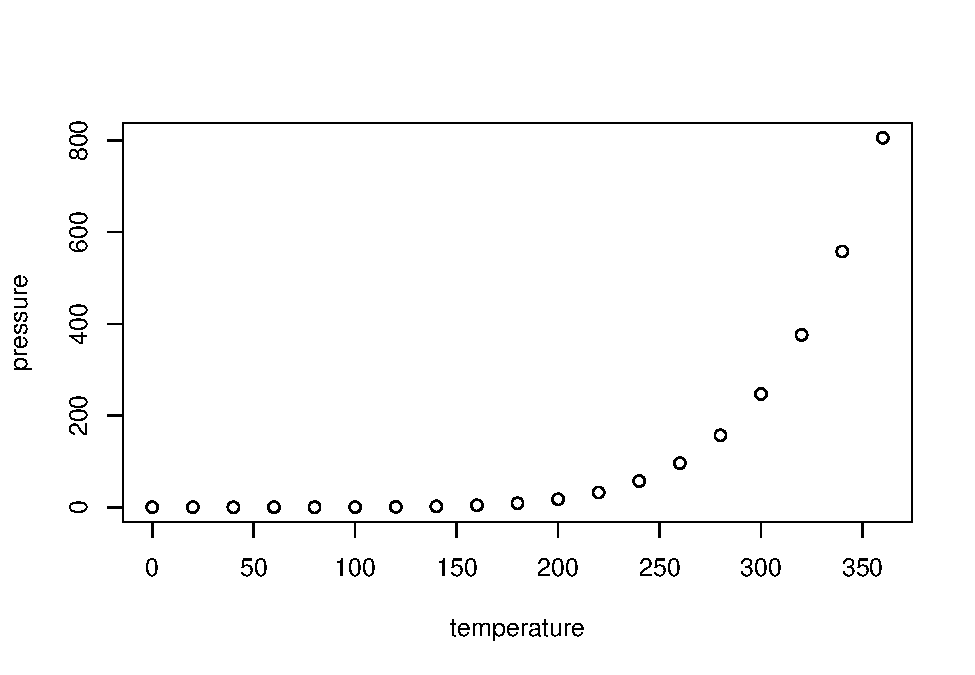
\includegraphics{StreamFluxArticle_files/figure-latex/unnamed-chunk-2-1} \caption{Please caption every figure}\label{fig:unnamed-chunk-2}
\end{figure}

Example table

\begin{table}
 \caption{Time of the Transition Between Phase 1 and Phase 2$^{a}$}
 \centering
 \begin{tabular}{l c}
 \hline
  Run  & Time (min)  \\
 \hline
   $l1$  & 260   \\
   $l2$  & 300   \\
   $l3$  & 340   \\
   $h1$  & 270   \\
   $h2$  & 250   \\
   $h3$  & 380   \\
   $r1$  & 370   \\
   $r2$  & 390   \\
 \hline
 \multicolumn{2}{l}{$^{a}$Footnote text here.}
 \end{tabular}
 \end{table}

AGU prefers the use of \{sidewaystable\} over \{landscapetable\} as it
causes fewer problems.

\begin{sidewaysfigure}[h]
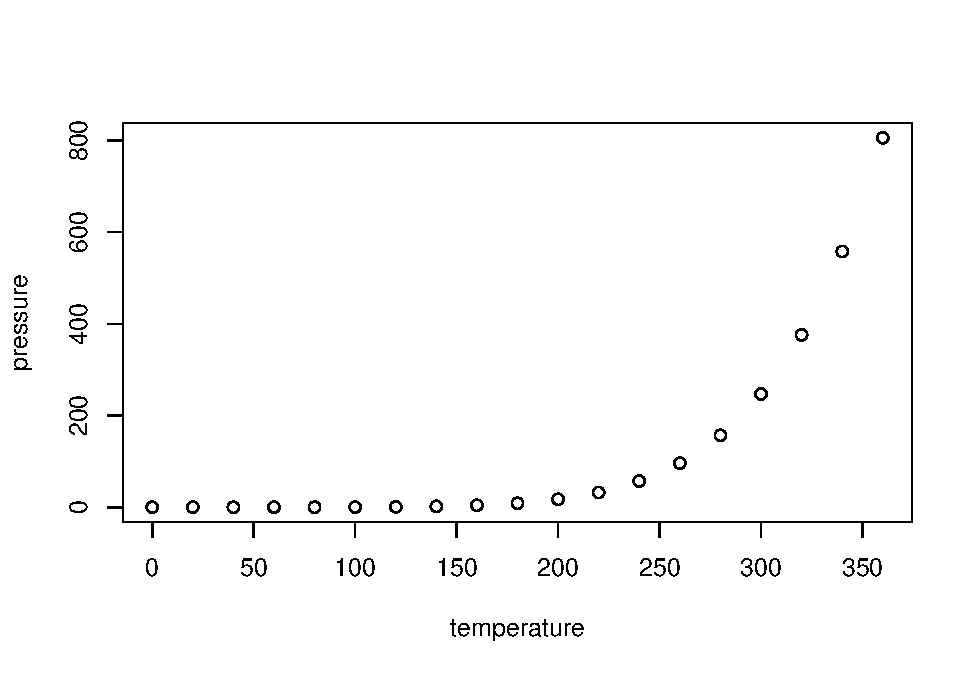
\includegraphics{StreamFluxArticle_files/figure-latex/unnamed-chunk-3-1} \caption{Please caption every figure}\label{fig:unnamed-chunk-3}
\end{sidewaysfigure}

\begin{sidewaystable}
\caption{Caption here}
\label{tab:signif_gap_clos}
\begin{tabular}{ccc}
one&two&three\\
four&five&six
\end{tabular}
\end{sidewaystable}

If using numbered lines, please surround equations with
\textbackslash{}begin\{linenomath*\}\ldots{}
\textbackslash{}end\{linenomath*\}

\begin{linenomath*}
\begin{equation}
y|{f} \sim g(m, \sigma)
\end{equation}
\end{linenomath*}

\section{Conclusions}

\appendix
\section{Here is a sample appendix}

Optional Appendix goes here

Optional Glossary, Notation or Acronym section goes here:

Glossary is only allowed in Reviews of Geophysics

\begin{glossary}
\term{Term}
 Term Definition here
\term{Term}
 Term Definition here
\term{Term}
 Term Definition here
\end{glossary}

\begin{acronyms}
\acro{Acronym}
 Definition here
\acro{EMOS}
 Ensemble model output statistics
\acro{ECMWF}
 Centre for Medium-Range Weather Forecasts
\end{acronyms}

\begin{notation}
\notation{$a+b$} Notation Definition here
\notation{$e=mc^2$}
Equation in German-born physicist Albert Einstein's theory of special
relativity that showed that the increased relativistic mass ($m$) of a
body comes from the energy of motion of the body—that is, its kinetic
energy ($E$)—divided by the speed of light squared ($c^2$).
\end{notation}

\acknowledgments

The acknowledgments must list: A statement that indicates to the reader
where the data supporting the conclusions can be obtained (for example,
in the references, tables, supporting information, and other databases).

All funding sources related to this work from all authors

Any real or perceived financial conflicts of interests for any author

Other affiliations for any author that may be perceived as having a
conflict of interest with respect to the results of this paper.

It is also the appropriate place to thank colleagues and other
contributors.

AGU does not normally allow dedications.

\bibliography{agutest.bib}


\end{document}
